\chapter{Unfortunately the op-amp is not so ideal}
In this set of experiments we dealt with the problems of a real op-amp such as the offset $v_{os}$, the bias currents $i_{b+},i_{b-}$, the slew-rate, the maximum current output and the common gain $A_{cm}$: we performed the measures of these real parameters. The offset is studied with 3 different circuits and then compensated with a trimmer in the configuration suggested by the op-amp's datasheet. The bias currents were measured in two ways, one for the bias current in the non inverting op-amp input and one for the inverting one. The other parameters are studied simply adjusting the input for the measurement's purpose.

\section{Materials}
\begin{itemize}
\item Operational amplifier uA741
\item Resistors, trimmers and capacitors
\item Power supply RIGOL DP831A
\item Waveform generator RIGOL DG1032
\item Multimeter RIGOL DM3068
\item Oscilloscope RIGOL MS02102A
\end{itemize}
\begin{table}[H]
\centering
\begin{tabular}{ |p{3cm}||p{3cm}|p{3cm}| }
 \hline
 \multicolumn{3}{|c|}{List of resistors used} \\
 \hline
 Resistor name & Value [$\Omega$] & Uncertainty [$\Omega$]\\
 \hline
 R$_{\text{M}\Omega}$   & 982.0 $\times$ 10$^3$ & 0.1 $\times$ 10$^3$  \\
 R$_{100\text{k}\Omega}$& 99.22 $\times$ 10$^3$ & 0.01 $\times$ 10$^3$ \\
 R$_{10\text{k}\Omega}$ &   9906.2            & 1.2         \\
 R$_{\text{k}\Omega}$   &  1001.4             & 0.1         \\
 R$_{10\Omega}$         &  9.963              & 0.01        \\
 R$_{10\text{k}\Omega}^*$ &  9926.4             & 1.2         \\
 R$_{10\Omega}^*$       &10.00                & 0.01        \\ 
 \hline
\end{tabular}
\end{table}

\section{Experiment setup}
In all the circuits we placed on the power supply's pins two capacitors each, one with high capacitace (nominal value 470 $\pm$ 23 nF) and one with low capacitance (10.0 $\pm$ 0.5 nF). These were used for suppressing the high-frequency noise and contrasting the effect of any eventual change in the power supply voltage, that could move the offset voltage.
\begin{figure}[H]
\centering
\begin{minipage}{.32\textwidth}
  \centering
  \begin{circuitikz}
 	\draw(0,0) node[op amp] (opamp) {}
	%(opamp.+) node[left] {$v_+$}
	(opamp.-) ++ (-.3,0) -- (opamp.-) 
	(opamp.-) ++ (-.3,0) -- (-1.5,1.8) -- (1.6,1.8) -- (1.6,0)
	(opamp.out) to [short,-o](1.8,0) node[right] {$v_o$}
	(opamp.up) ++(0,.5) node[above] {$+v_{cc}$} -- (opamp.up)
	(opamp.down) ++ (0,-.5) node[below] {$-v_{cc}$} -- (opamp.down)
	(opamp.down) ++ (0,-.25)to[C,/tikz/circuitikz/bipoles/length=1cm] (1,-.8)node[ground,rotate = 90,yshift = 1em] {}
	(opamp.up) ++ (0,.25)to[C,/tikz/circuitikz/bipoles/length=1cm] (1,.8)node[ground,rotate = 90,yshift = 1em] {};
	\draw(opamp.+) ++ (-.3,0)node[ground] {} -- (opamp.+);
	\end{circuitikz}
\caption{Offset voltage's direct measure}\label{offset direct}
\end{minipage}%
\begin{minipage}{.32\textwidth}
  \centering
  \begin{circuitikz}
\draw(0,0) node[op amp] (opamp) {}
	%(opamp.+) node[left] {$v_+$}
	(opamp.+) ++ (-.3,0) node[ground] {} -- (opamp.+) 
	(opamp.out) to [short,-o](1.8,0) node[right] {$v_o$}
	(opamp.down) ++(0,-.5) node[below] {$-v_{cc}$} -- (opamp.down)
	(opamp.up) ++ (0,.5) node[above] {$+v_{cc}$} -- (opamp.up)
	(opamp.down) ++ (0,-.25)to[C,/tikz/circuitikz/bipoles/length=1cm] (1,-.8)node[ground,rotate = 90,yshift = 1em] {}
	(opamp.up) ++ (0,.25)to[C,/tikz/circuitikz/bipoles/length=1cm] (1,.8)node[ground,rotate = 90,yshift = 1em] {};
	\draw(-3.1,.5) to[R,l=R$_{10\Omega}$] (-1.5,.5) to[short] (opamp.-);
	\draw(-3.1,.5) node[ground] {};
	\draw(-1.5,.5) to[short](-1.5,2.2) to[R,l=R$_{10\text{k}\Omega}$](1.5,2.2) to[short](1.5,0);
\end{circuitikz}
\caption{Offset voltage's direct measure with gain}\label{offset amp}
\end{minipage}%
\begin{minipage}{.32\textwidth}
  \centering
\begin{circuitikz}
\draw(0,0) node[op amp] (opamp) {}
	%(opamp.+) node[left] {$v_+$}
	%(opamp.+) ++ (-.3,0) node[ground] {} -- (opamp.+) 
	(opamp.out) to [short,-o](1.8,0) node[right] {$v_o$}
	(opamp.down) ++(0,-.5) node[below] {$-v_{cc}$} -- (opamp.down)
	(opamp.up) ++ (0,.5) node[above] {$+v_{cc}$} -- (opamp.up)
	(opamp.down) ++ (0,-.25)to[C,/tikz/circuitikz/bipoles/length=1cm] (1,-.8)node[ground,rotate = 90,yshift = 1em] {}
	(opamp.up) ++ (0,.25)to[C,/tikz/circuitikz/bipoles/length=1cm] (1,.8)node[ground,rotate = 90,yshift = 1em] {};
	\draw(-3,.5) to[R,l=R$_{10\Omega}$] (-1.5,.5) to[short] (opamp.-);
	\draw(-3,.5) node[ground] {};
	\draw(-1.5,.5) to[short](-1.5,2.2) to[R,l=R$_{10\text{k}\Omega}$](1.5,2.2) to[short](1.5,0);
	
	\draw(opamp.+) to[short](-1.7,-.5)to[short](-1.7,-1) to[short](-2.1,-1) to[R,l_=R$^*_{10\text{k}\Omega}$](-2.1,-3)to[short](-1.7,-3)node[ground]{};
	\draw(-1.7,-1)to[short](-1.3,-1)to[R,l=R$^*_{10\Omega}$](-1.3,-3)to[short](-1.7,-3);
\end{circuitikz}
\caption{Offset voltage's direct measure with gain and bias current correction}\label{offset amp corrected}
\end{minipage}
\end{figure}
In the first circuit we aquired $v_{os}$ directly by measuring with the multimiter a follower output voltage.
We used the second circuit drawn to amplify $v_{os}$, thus we measured the output to calculate $v_{os}$.\\
The third circuit is identical to  the second except for the added resistors in parallel that connect the non inverting pin to the ground: this was done for removing the bias current influence from the measurament according to the hypothesis that these currents are similar to each other. For that reason these added resistors must have toghether the same resistance of the parallel between the $R_{10 \Omega}$ and $R_{10 k\Omega}$ used before.\ Exploiting this last circuit we removed $v_{os}$ by using a trimmer between op-amp pins 1 and 5, paying attention to connect the central trimmer pin to the negative power supply voltage (according to the uA741 datasheet): we tried to make the output as close to 0 as possible (we used no input voltage in these steps).
\begin{figure}[H]
\centering
\begin{minipage}{.5\textwidth}
  \centering
\begin{circuitikz}
\draw(0,0) node[op amp] (opamp) {}
	%(opamp.+) node[left] {$v_+$}
	%(opamp.+) ++ (-.3,0) node[ground] {} -- (opamp.+) 
	(opamp.out) to [short,-o](1.8,0) node[right] {$v_o$}
	%(opamp.down) ++(0,-.5) node[below] {$-v_{cc}$} -- (opamp.down)
	(opamp.up) ++ (0,.5) node[above] {$+v_{cc}$} -- (opamp.up)
	(opamp.down) ++ (0,-.25)to[C,/tikz/circuitikz/bipoles/length=1cm] (1,-.8)node[ground,rotate = 90,yshift = 1em] {}
	(opamp.up) ++ (0,.25)to[C,/tikz/circuitikz/bipoles/length=1cm] (1,.8)node[ground,rotate = 90,yshift = 1em] {};
	\draw(-3.5,.5) to[R,l=R$_{\text{k}\Omega}$] (-1.5,.5) to[short] (opamp.-);
	\draw(-3.5,.5) node[ground] {};
	\draw(-1.5,.5) to[short](-1.5,2.2) to[R,l=R$_{100\text{k}\Omega}$](1.5,2.2) to[short](1.5,0);
	\draw(opamp.+) to[short](-1.2,-.5)to[R,l_=R$_{\text{M}\Omega}$](-1.2,-2.5)node[ground]{};
	\draw(opamp.down) ++ (-.45,-.25)to[short](-0.53,-2)to[R](1.53,-2);
	\draw(opamp.down) ++ (.6,.36) to[short](.515,-.35) to[short](1.53,-.35) to[short](1.53,-2);	
	\draw(opamp.down) to [short](-.085,-1.3)to[short](.42,-1.3);	
	\draw(-.085,-1.3) to[short](-.085,-1.45)node[below]{\scriptsize$-v_{cc}$};
	\draw[-stealth](.415,-1.3) -- (.415,-1.76);
\end{circuitikz}
\caption{Positive bias current measure}\label{current positive}
\end{minipage}%
\begin{minipage}{.5\textwidth}
\centering
\begin{circuitikz}
\draw(0,0) node[op amp] (opamp) {}
	%(opamp.+) node[left] {$v_+$}
	(opamp.+) ++ (-.3,0) node[ground] {} -- (opamp.+) 
	(opamp.out) to [short,-o](1.8,0) node[right] {$v_o$}
	%(opamp.down) ++(0,-.5) node[below] {$-v_{cc}$} -- (opamp.down)
	(opamp.up) ++ (0,.5) node[above] {$+v_{cc}$} -- (opamp.up)
	(opamp.down) ++ (0,-.25)to[C,/tikz/circuitikz/bipoles/length=1cm] (1,-.8)node[ground,rotate = 90,yshift = 1em] {}
	(opamp.up) ++ (0,.25)to[C,/tikz/circuitikz/bipoles/length=1cm] (1,.8)node[ground,rotate = 90,yshift = 1em] {};
	\draw(-5,.49) to[R,l=R$_{\text{k}\Omega}$] (-3,.49) to[R,l=R$_{100\text{k}\Omega}$](-1,.49);%to[short](opamp.-);
	\draw(-5,.49) node[ground] {};
	\draw(-3,.49) to[short](-3,2.2) to[R,l=R$_{\text{M}\Omega}$](1.5,2.2) to[short](1.5,0);
	%\draw(opamp.+) to[short](-1.2,-.5)node[ground]{};
	\draw(opamp.down) ++ (-.45,-.25)to[short](-0.53,-2)to[R](1.53,-2);
	\draw(opamp.down) ++ (.6,.36) to[short](.515,-.35) to[short](1.53,-.35) to[short](1.53,-2);	
	\draw(opamp.down) to [short](-.085,-1.3)to[short](.42,-1.3);
	\draw(-.085,-1.3) to[short](-.085,-1.45)node[below]{\scriptsize$-v_{cc}$};
	\draw[-stealth](.415,-1.3) -- (.415,-1.76);
\end{circuitikz}
\caption{Negative bias current measure}\label{current negative}
\end{minipage}
\end{figure}
The fourth circuit and the fifth are used for measuring the bias currents indirectly basing on how the two currents are related to the output: we use a great resistance ($R_{M\Omega}$) in order to make relevant to a voltage measurement only one bias current with respect to the other.\\
The sixth circuit was used for measuring the maximum current that the op-amp can erogate. In this configuration the oscilloscope's internal resitor was set to $50 \Omega$.\\
\begin{figure}[H]
\centering
\begin{minipage}{.5\textwidth}
\centering
\begin{circuitikz}
 	\draw(0,0) node[op amp] (opamp) {}
	%(opamp.+) node[left] {$v_+$}
	(opamp.-) ++ (-.3,0) -- (opamp.-) 
	(opamp.-) ++ (-.3,0) -- (-1.5,1.8) -- (1.6,1.8) -- (1.6,0)
	(opamp.out) to [short](2.5,0)to[myvoltmeter,l=Oscilloscope $50\ohm$](2.5,-1.5)node[ground]{}
	(opamp.up) ++(0,.5) node[above] {$+v_{cc}$} -- (opamp.up)
	(opamp.down) ++ (0,-.25)to[C,/tikz/circuitikz/bipoles/length=1cm] (1,-.8)node[ground,rotate = 90,yshift = 1em] {}
	(opamp.up) ++ (0,.25)to[C,/tikz/circuitikz/bipoles/length=1cm] (1,.8)node[ground,rotate = 90,yshift = 1em] {};
	%\draw(opamp.+) ++ (-.3,0)node[ground] {} -- (opamp.+);
	\draw(opamp.down) ++ (-.45,-.25)to[short](-0.53,-2)to[R](1.53,-2);
	\draw(opamp.down) ++ (.6,.36) to[short](.515,-.35) to[short](1.53,-.35) to[short](1.53,-2);
	\draw(opamp.down) to [short](-.085,-1.3)to[short](.42,-1.3);
	\draw(-.085,-1.3) to[short](-.085,-1.45)node[below]{\scriptsize$-v_{cc}$};
	\draw[-stealth](.415,-1.3) -- (.415,-1.76);
	\draw(-2,-2)node[ground]{}to[tV](-2,-.5) -- (opamp.+);
	\draw(2.5,0)to[short,-o](2.8,0)node[right] {$v_o$};
	\end{circuitikz}
	\caption{Max current measure}\label{max current}
\end{minipage}%
\begin{minipage}{.5\textwidth}
\centering
\begin{circuitikz}
 	\draw(0,0) node[op amp] (opamp) {}
	%(opamp.+) node[left] {$v_+$}
	(opamp.-) ++ (-.3,0) -- (opamp.-) 
	(opamp.-) ++ (-.3,0) -- (-1.5,1.8) -- (1.6,1.8) -- (1.6,0)
	(opamp.out) to [short](2.5,0)to[short](2.5,-.3)to[short](2.2,-.3)to[C](2.2,-1.8)to[short](2.5,-1.8)node[ground]{}
	(opamp.up) ++(0,.5) node[above] {$+v_{cc}$} -- (opamp.up)
	(opamp.down) ++ (0,-.25)to[C,/tikz/circuitikz/bipoles/length=1cm] (1,-.8)node[ground,rotate = 90,yshift = 1em] {}
	(opamp.up) ++ (0,.25)to[C,/tikz/circuitikz/bipoles/length=1cm] (1,.8)node[ground,rotate = 90,yshift = 1em] {};
	%\draw(opamp.+) ++ (-.3,0)node[ground] {} -- (opamp.+);
	\draw(opamp.down) ++ (-.45,-.25)to[short](-0.53,-2)to[R](1.53,-2);
	\draw(opamp.down) ++ (.6,.36) to[short](.515,-.35) to[short](1.53,-.35) to[short](1.53,-2);
	\draw(opamp.down) to [short](-.085,-1.3)to[short](.42,-1.3);
	\draw(-.085,-1.3) to[short](-.085,-1.45)node[below]{\scriptsize$-v_{cc}$};
	\draw[-stealth](.415,-1.3) -- (.415,-1.76);
	\draw(-2,-2)node[ground]{}to[sqV](-2,-.5) -- (opamp.+);
	\draw(2.5,0)to[short,-o](2.8,0)node[right] {$v_o$};
	\draw(2.5,-.3)to[short](3,-.3)to[R](3,-1.8)to[short](2.5,-1.8);
	\end{circuitikz}
	\caption{Slew rate}\label{slew rate}
\end{minipage}
\end{figure}
With the seventh circuit we measured the slew rate: the load capacitor used was 1 $\pm$ 0.05 nF, the resistor 2 $\pm$ 0.1 k$\Omega$ and the input used a 0-10 V square wave, that allowed us to aquire the image of the raising output.\\
Finally, the last circuit allowed us to measure the common gain by using the differential amplifier with the same 2V peak-peak sine signal at 100 Hz as the two inputs.\\
\begin{figure}[H]
\centering
\begin{circuitikz}
\draw(0,0) node[op amp] (opamp) {}
	%(opamp.+) node[left] {$v_+$}
	%(opamp.+) ++ (-.3,0) node[ground] {} -- (opamp.+) 
	(opamp.out) to [short,-o](1.8,0) node[right] {$v_o$}
	(opamp.up) ++ (0,.5) node[above] {$+v_{cc}$} -- (opamp.up)
	(opamp.down) ++ (0,-.25)to[C,/tikz/circuitikz/bipoles/length=1cm] (1,-.8)node[ground,rotate = 90,yshift = 1em] {}
	(opamp.up) ++ (0,.25)to[C,/tikz/circuitikz/bipoles/length=1cm] (1,.8)node[ground,rotate = 90,yshift = 1em] {};
	\draw(-3.5,.5) to[R=$R_1$] (-1.5,.5) to[short] (opamp.-);
	\draw(-3.5,.5) to[short](-3.5,-.5);
	\draw(-1.5,.5) to[short](-1.5,2.2) to[R=$R_f$](1.5,2.2) to[short](1.5,0);
	\draw(-3.5,-.5) to[R=$R_1||R_f$] (-1.5,-.5) to[short] (opamp.+);
	\draw(-3.5,-.5) to[sV](-3.5,-2)node[ground]{};
	\draw(opamp.down) ++ (-.45,-.25)to[short](-0.53,-2)to[R](1.53,-2);
	\draw(opamp.down) ++ (.6,.36) to[short](.515,-.35) to[short](1.53,-.35) to[short](1.53,-2);
	\draw(opamp.down) to [short](-.085,-1.3)to[short](.42,-1.3);
	\draw(-.085,-1.3) to[short](-.085,-1.45)node[below]{\scriptsize$-v_{cc}$};
	\draw[-stealth](.415,-1.3) -- (.415,-1.76);
\end{circuitikz}
\caption{Common Gain}\label{common gain}
\end{figure}

\section{Data analysis}
In the emitter follower \eqref{offset direct} the output measured is $-1.484 \pm 0.005$ mV. Being such a small output we expect to have problems with parassite impedance and other forms of noise, that's why we don't consider the output too reliable. It however gives us an order of magnitude that matches the op-amp datasheet, acording to which absolute typical values are from 1 mV to 5 mV.\\
In the amplifier \eqref{offset amp} we can find $v_{os}$ resolving
\[v_{os} = \frac{v_{o}}{1 + \frac{R_{10\text{k}\Omega}}{R_{10\Omega}}}\]
From the calculation we get $v_{os} = -1.333 \pm 0.001$ mV, which has the same order of magnitude and sign of the previous result.\\
Then, as stated in the experimental setup, we corrected the circuit \eqref{offset amp corrected} for compensating the bias currents effect. With the same formula used for the previous amplifier we got an offset voltage of $1.307 \pm 0.001$ mV.\\
At this point we compensated the offset through the use of a trimmer (see experimental setup).\\
Reguarding the fourth circuit \eqref{current positive}, we calculated the current flowing in the non invertent pin by using $$i_{b+} = -\frac{v_{o}}{R_{\text{M}\Omega} (1 + \frac{R_{100\text{k}\Omega}}{R_{1\text{k}\Omega}})}$$ The value calculated is $-39.042 \pm 0.009$ nA.\\
The fifth circuit \eqref{current negative} instead leads to the calculation of the current flowing in the invertent pin by using 
\[i_{b-} = \frac{v_{o}}{R_{100\text{k}\Omega}} \frac{R_{\text{k}\Omega}}{R_{\text{M}\Omega}}\]
we obtain the value $-39.724 \pm 0.009$ nA. Now we can compute the bias current $i_b = \frac{|i_{b-}| + |i_{b+}|}{2} = 39.383 \pm 0.006$ nA and the offset current $i_o = ||i_{b-}| - |i_{b+}|| = 0.68 \pm 0.01$ nA.\\
$i_b$ is less than 100 nA and near the typical value of 10 nA, as the datasheet states, but the offset current is a bit low being around a third of the typical value 2 nA.\\
\begin{figure}[H]
\centering
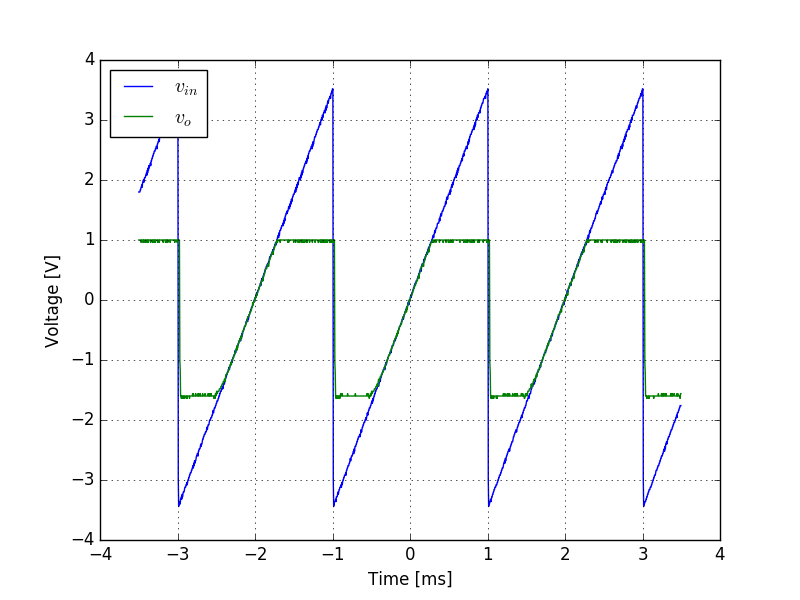
\includegraphics[width=.6\textwidth]{3/Maximum_current_erogated.png}
\caption{Saturated output caused by the maximum current erogated}
\end{figure}
In the sixth circuit \eqref{max current} we calculated the maximum current erogated by computing the maximum/minimum output voltage over the resistance in the oscilloscope. In the plot is visible the different absolute value of the maximum and minimum output voltage, that's probably because the op-amp isn't perfectly symmetric in the packaging. So we chose to calculate two different maximum currents: $i_{max} = 0.0201 \pm 0.0001$ A (when the output was positive) and $i_{min} = -0.0328 \pm 0.0001$ (when the output was negative).
\begin{figure}[H]
\centering
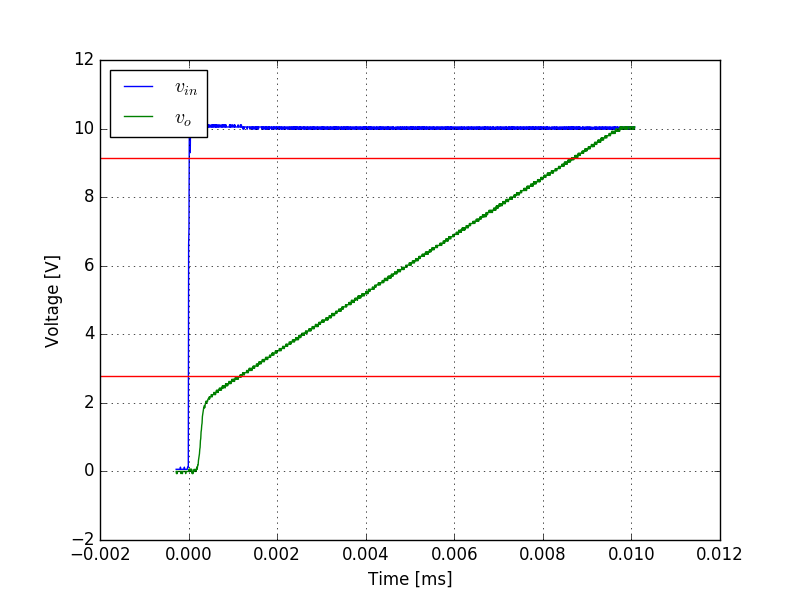
\includegraphics[width=.6\textwidth]{3/Slew_Ratio.png}
\caption{Saturated output caused by the maximum current erogated, red lines is 10\% and 90\% of the output}
\end{figure}
In the seventh circuit \eqref{slew rate} we find that the slew rate ($\frac{\Delta V}{\Delta t}$) of the op-amp used is $0.8332 \pm 0.0026 \frac{\text{V}}{\mu s}$, which is bigger than the typical value $0.5 \frac{\text{V}}{\mu s}$. One possible explenation of this would be that the slew rate depends on the amplitude of the signal: in our experiment the voltage was 50 times larger than the test shown in the datasheet, otherwise we have to conclude that our op-amp, has some difects that cause a larger slew rate.
\begin{figure}[H]
\centering
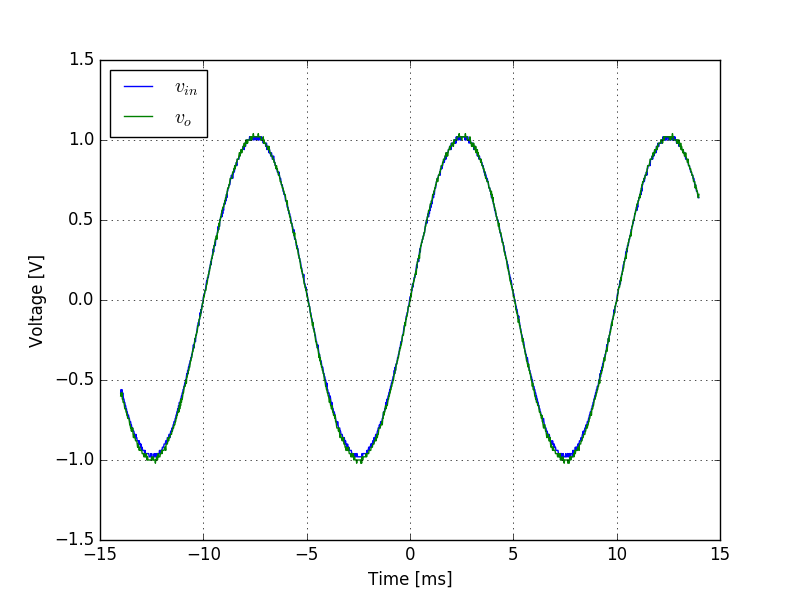
\includegraphics[width=.7\textwidth]{3/Amplification_in_common_mode.png}
\caption{Saturated output caused by the maximum current erogated}
\end{figure}
With the last circuit \eqref{common gain} we measured the common gain of our op-amp, by solving
\[A_{CM} = \frac{2 v_{o}}{v_{in1} + v_{in2}}\]
which gave us an unitary gain, as it is evident in the plot.
